\documentclass{article}
\usepackage[german]{babel}
\usepackage{float}
\usepackage{fourier}
\usepackage[utf8]{inputenc}
\usepackage[T1]{fontenc}
\usepackage{amsfonts,amsthm, amsmath}
\usepackage{listings}
% The following is needed in order to make the code compatible
% with both latex/dvips and pdflatex.
\ifx\pdftexversion\undefined
\usepackage[dvips]{graphicx}
\else
\usepackage[pdftex]{graphicx}
\DeclareGraphicsRule{*}{mps}{*}{}
\fi

\setlength\parindent{0pt}
\lstset{language=Erlang}

\begin{document}

\textbf{Team:} Falco Winkler (FW), Daniel Schruhl (DS)\\
\\
\textbf{Aufgabenteilung:}\\

\textbf{Quellenangaben:}\\
\\
\textbf{Bearbeitungszeitraum:}
\begin{itemize}
	\item 26.03.2017 (FW,DS)
\end{itemize}

\textbf{Aktueller Stand:}\\

\textbf{Änderung des Entwurfs:}\\
-

\newpage
\tableofcontents 
\newpage

\section{Einführung und Ziele}
Es soll eine Message of the Day Anwendung erstellt werden. Dabei werden von verschiedenen Clients an einen Server verschiedene Nachrichten des Tages gesendet. Die Clients rufen vom Server alle Nachrichten ab, so dass jeder Client alle Nachrichten in einer festen Reihenfolge hat.

\subsection{Randbedingungen}
Es soll eine Client/Server-Architektur implementiert werden.
Der Server verwaltet dabei die ihm von den Clients gesendeten Nachrichten. Das beinhaltet eine feste Numerierung der Nachrichten.

Die Clients rufen dabei in bestimmten Abständen die Nachrichten ab. Falls ein Client dem Server schon bekannt ist, bekommt der nur die ihm noch unbekannten (neuen) Nachrichten.

Der Server muss sich also die Clients merken. Es soll mit einer Holdbackqueue und einer Deliveryqueue gearbeitet werden, um die korrekte Auslieferung in einer bestimmten Reihenfolge der Nachrichten zu garantieren.

\subsection{Kontextbegrenzung}
Das System soll in Erlang umgesetzt werden. Es muss auf Computern mit Linux Betriebssystem lauffähig sein.

\newpage

\section{Gesamtsystem}
\subsection{Kontextsicht}
\subsection{Bausteinsicht}
\subsection{Laufzeitsicht}
\subsection{Verteilungssicht}
\subsection{Konfigurationsparameter}
\subsection{Benutzungsschnittstelle}


	\subsection{Architekturüberblick}
	Komponentendiagramm
	\begin{figure}[H]
	\centering
		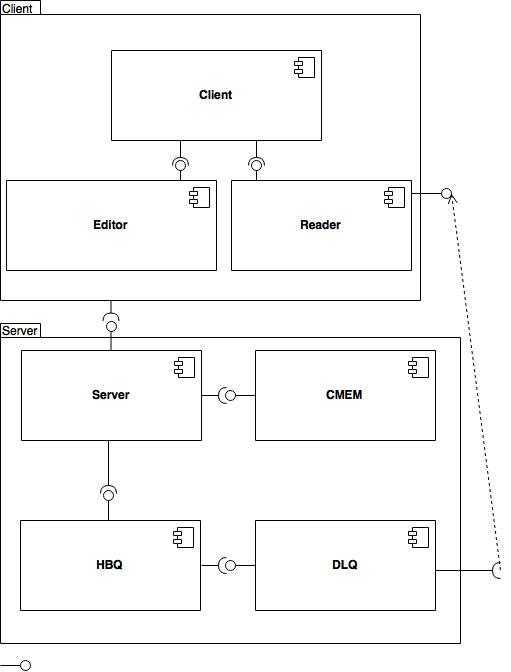
\includegraphics[width=\textwidth]{component-diagram.png}
	\caption[seq-dia]{Komponentendiagramm der Message Of The Day App}
	\label{fig:component-diagram}
	\end{figure}

	Das Softwareprodukt besteht aus mehreren Modulen und Paketen. Das Client-Paket und das Server-Paket.

	Im Server Paket befinden sich das Server-Modul und alle vom Server-Modul verwendeten Datenstrukturen in Modulen.
	Dazu gehören das HBQ-Modul, das DLQ-Modul und das CMEM-Modul.

	Die Schnittstellen des DLQ-Moduls und CMEM-Moduls sind als RPC implementiert. Die Schnittstellen des HBQ-Moduls und des
	Server-Moduls sind als entfernte ADT realisiert.

	Die DLQ Schnittstelle wird nur von der HBQ konsumiert und die CMEM Schnittstelle wird nur vom Server konsumiert.
	Die Schnittstelle der HBQ wird nur vom Server verwendet und die Schnittstelle vom Server ist nur an den Client angebunden.

	Das Client-Paket beinhaltet die Client-Module. Diese sind zum einen der Lese Client (Reader-Modul) und der Redakteur
	Client (Editor-Modul). Beide Clients sind als ein Prozess implementiert.
	
	\textbf{Entwurf:}\\
Sequenzdiagramm
\begin{figure}[H]
\centering
	\includegraphics[width=\textwidth]{sequence-diagram.png}
\caption[seq-dia]{Sequenzdiagramm bei fehlerfreiem Nachrichtenaustausch}
\label{fig:sequence-diagram}
\end{figure}


\section{Subsysteme und Komponenten}
	\subsection{Client}
		\subsubsection{Aufgabe und Verantwortung des Clients}
			Der Client ist ein einzelner Prozess, der sich jedoch in zwei Rollen aufteilt. 
			Im Endlosdurchlauf einer Schleife wechselt er zwischen 
			Leser und Redakteur - Rolle.
        		\newline
			Der Client wird in drei Module aufgespalten: Client, Reader und Writer. 
			Client ruft in einer Endlosschleife wechselweise die soeben beschriebene 
			Funktionalität in den Modulen Reader und Writer auf.
		\subsubsection{Entwurfsentscheidungen}
		\subsubsection{Außensicht}
		\subsubsection{Innensicht}
		\subsubsection{Konfigurationsparameter}
    	\subsubsection{Komponente Leserclient}
    	
    		\paragraph{Aufgabe und Verantwortung des Leseclients}
    		Der Leseclient liest solange Nachrichten vom Server, 
    		bis keine weiteren Nachrichten mehr vorhanden sind.
			\paragraph{Entwurfsentscheidungen}
			\paragraph{Außensicht}
			\paragraph{Innensicht}
			\paragraph{Konfigurationsparameter}
		
		\subsubsection{Komponente Redakteurclient}
		
		    \paragraph{Aufgabe und Verantwortung des Redakteurclients}
		    Der Redakteurclient sendet fünf Nachrichten an den Server, 
		    und fragt danach einmal die nächste NNr ab, um eine Lücke in den fortlaufend 
		    nummerierten Nachrichten zu produzieren.
			\paragraph{Entwurfsentscheidungen}
			\paragraph{Außensicht}
			\paragraph{Innensicht}
			\paragraph{Konfigurationsparameter}
			
	\subsection{Server}
	
		\subsubsection{Aufgabe und Verantwortung des Servers}
			Der Server hat die Aufgaben  
			\begin{enumerate}
    			\item{Sich anfragende Clients mit ProzessID und Zeitstempel zu merken}
    			\item{Clients die ihnen zugehörigen Nachrichten zurückzugeben}
			\end{enumerate}
			Für die erste Aufgabe wird das Modul CMEM verwendet. 
			Zum Senden an die Clients leitet der Server die Nachrichten zunächst an die HBQ weiter. 
			Erscheint eine Anfrage vom Client, erfolgt über die HBQ der Aufruf an die DLQ, 
			die Nachricht zu übermitteln.
		\subsubsection{Entwurfsentscheidungen}
		\subsubsection{Außensicht}
		\subsubsection{Innensicht}
		\subsubsection{Konfigurationsparameter}
		\subsubsection{Benutzungsschnittstelle}
		
		\subsubsection{Komponente CMEM}
			\paragraph{Aufgabe und Verantwortung der CMEM}
				Dieses Modul hat die Aufgabe sich anfragende Clients mittels einer ProzessID und eines Zeitstempels in einer Map-Datenstruktur zu merken, und diese für den Server bereitzustellen.
			\paragraph{Entwurfsentscheidungen}
			\paragraph{Außensicht}
			\paragraph{Innensicht}
			\paragraph{Konfigurationsparameter}
			
			
		\subsubsection{Komponente HBQ}
			\paragraph{Aufgabe und Verantwortung der HBQ}
				Von Redakteur-Clients gesendete Nachrichten werden hier zwischengespeichert. Gibt es keine Lücke in der fortlaufenden Nummerierung der Nachrichten, werden Sie an die DLQ weitergeleitet. Bei einer Überfüllung der HBQ (2/3 der Maximalen Kapazität der DLQ) wird die älteste Lücke in den Nachrichten mit einer künstlichen Nachricht geschlossen, und es werden erneut alle Lückenlosen Nachrichten an die DLQ weitergeleitet. Die HBQ stellt nur ein Interface für den Server bereit.
			\paragraph{Entwurfsentscheidungen}
			\paragraph{Außensicht}
			\paragraph{Innensicht}
			\paragraph{Konfigurationsparameter}
			
		\subsubsection{Komponente DLQ}
			\paragraph{Aufgabe und Verantwortung der DLQ}
				Die Delivery - Queue hat die Aufgabe Nachrichten an Clients zuzustellen. 
				Die Nachrichten in der DLQ liegen immer sortiert vor, und es gibt keine Lücken in den NNr’s.
				Bei dem Sendevorgang erhält die DLQ ein Signal von der HBQ mit der PID des Ziel - Clients und der Nachrichtennummer. Daraufhin wird die Nachricht mit dieser NNr an den Client verschickt.
				Wenn diese Nachricht nicht vorhanden ist wird die Nachricht mit der nächst höheren NNr verschickt. 
				Es wird jeweils die Nummer der verschickten Nachricht zurückgegeben.
			\paragraph{Entwurfsentscheidungen}
			\paragraph{Außensicht}
			\paragraph{Innensicht}
			\paragraph{Konfigurationsparameter}


\end{document}